\documentclass[../notes.tex]{subfiles}
\graphicspath{
    {'../figures'}
}


\begin{document}

\banner{Fluid Mechanics}

\subsection{Density and Pressure}

\begin{definition}[Density]
    Density is the mass per unit volume:
    \[
        \boxed{
        \rho = \frac{m}{V} 
        }
    \]
    The units are $\qty[\rho] = \unit{kg/m^3}$.
\end{definition}

\begin{example}
    The first sphere has mass and radius $m$ and $R$ and the second $2m$ and $2R$ respectively. Since the volume of a sphere scale cubicaly, the spheres ratio of volumes are $\frac{1}{8}$ meaning the density of the first sphere is $\frac{1}{8}$ of the second.
    \begin{center}
        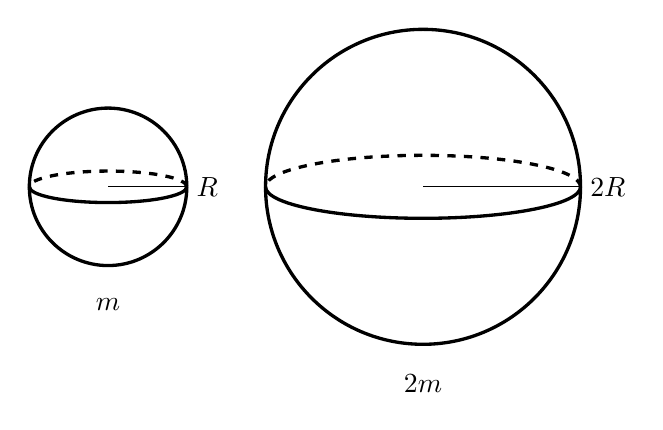
\begin{tikzpicture}
            \draw[very thick] (-2,0) circle[radius=1];
            \draw[very thick] (-3,0) arc (180:360:1 and 0.2);
            \draw[very thick, dashed] (-1,0) arc (0:180:1 and 0.2);
            \draw (-2,0) -- (-1,0) node[anchor=west] {$R$};
            \node at (-2,-1.5) {$m$};

            \draw[very thick] (2,0) circle[radius=2];
            \draw[very thick] (0,0) arc (180:360:2 and 0.4);
            \draw[very thick, dashed] (4,0) arc (0:180:2 and 0.4);
            \draw (2,0) -- (4,0) node[anchor=west] {$2R$};
            \node at (2,-2.5) {$2m$};

        \end{tikzpicture}
    \end{center}
\end{example}

Consider a fluid. That is, something that takes shape of the container it is in. Since it is in contact with the walls of the container, there is a normal force being exerted on the liquid by the container. This force is quantified by pressure

\begin{definition}[Pressure]
    Pressure is the magnitude of the normal force per unit area:
    \[
        \boxed{
        p = \frac{F_{\perp}}{A}
        }
    \]
    with units $\qty[p]= \unit{N / m^2} = \unit{Pa}$.
\end{definition}

\begin{example}
    Consider two evacuated discs pressed against each other with a vacuum in the middle. What is the force that holds them together? Each disk has a radius of $15 \unit{cm}$. Therefore the force on each one is
    \[
        F_{\perp} = p A = p_{\text{air}} \qty[\pi (0.15)^2]
    .\]
\end{example}

Pressure can also be expressed at a singular point in the form of a differential
\[
    p = \dv{F_{\perp}}{A}
.\]

\begin{theorem}[Pressure at Depth in a Fluid]
    The pressure at a depth inside of some fluid is
    \[
        \boxed{
        p = P_0 + \rho g k
        }
    .\]
    where $P_0$ is the pressure on the top surface of the fluid, $\rho$ the density of the fluid, and $k$ the depth that is being examined.
\end{theorem}

\begin{proof}
    % TODO :3
\end{proof}

\begin{theorem}[Pascals Law]
    \label{thm:pascals}
    A change in pressure at any point in an enclosed fluid at rest is transmitted undiminished to all points in the fluid.
\end{theorem}

\begin{theorem}[Archimedes Principle]
    \label{thm:archimedes}
    A body in a fluid experiences a bouyant force equal to the weight of fluid displaced. That is, the bouyant force is determined by the fluid element the body represents.
\end{theorem}

\end{document}
